
本项目紧密围绕实际需求开展研究,深入剖析当前已有方法在应对现实挑战时的局限性,旨在提出创新性研究方案,以攻克现存难题,总体研究思路如\reffig{fig:organization}所示,拟由此提升边防监控的智能化水平。

\begin{figure}[h!]
\centering %图片居中
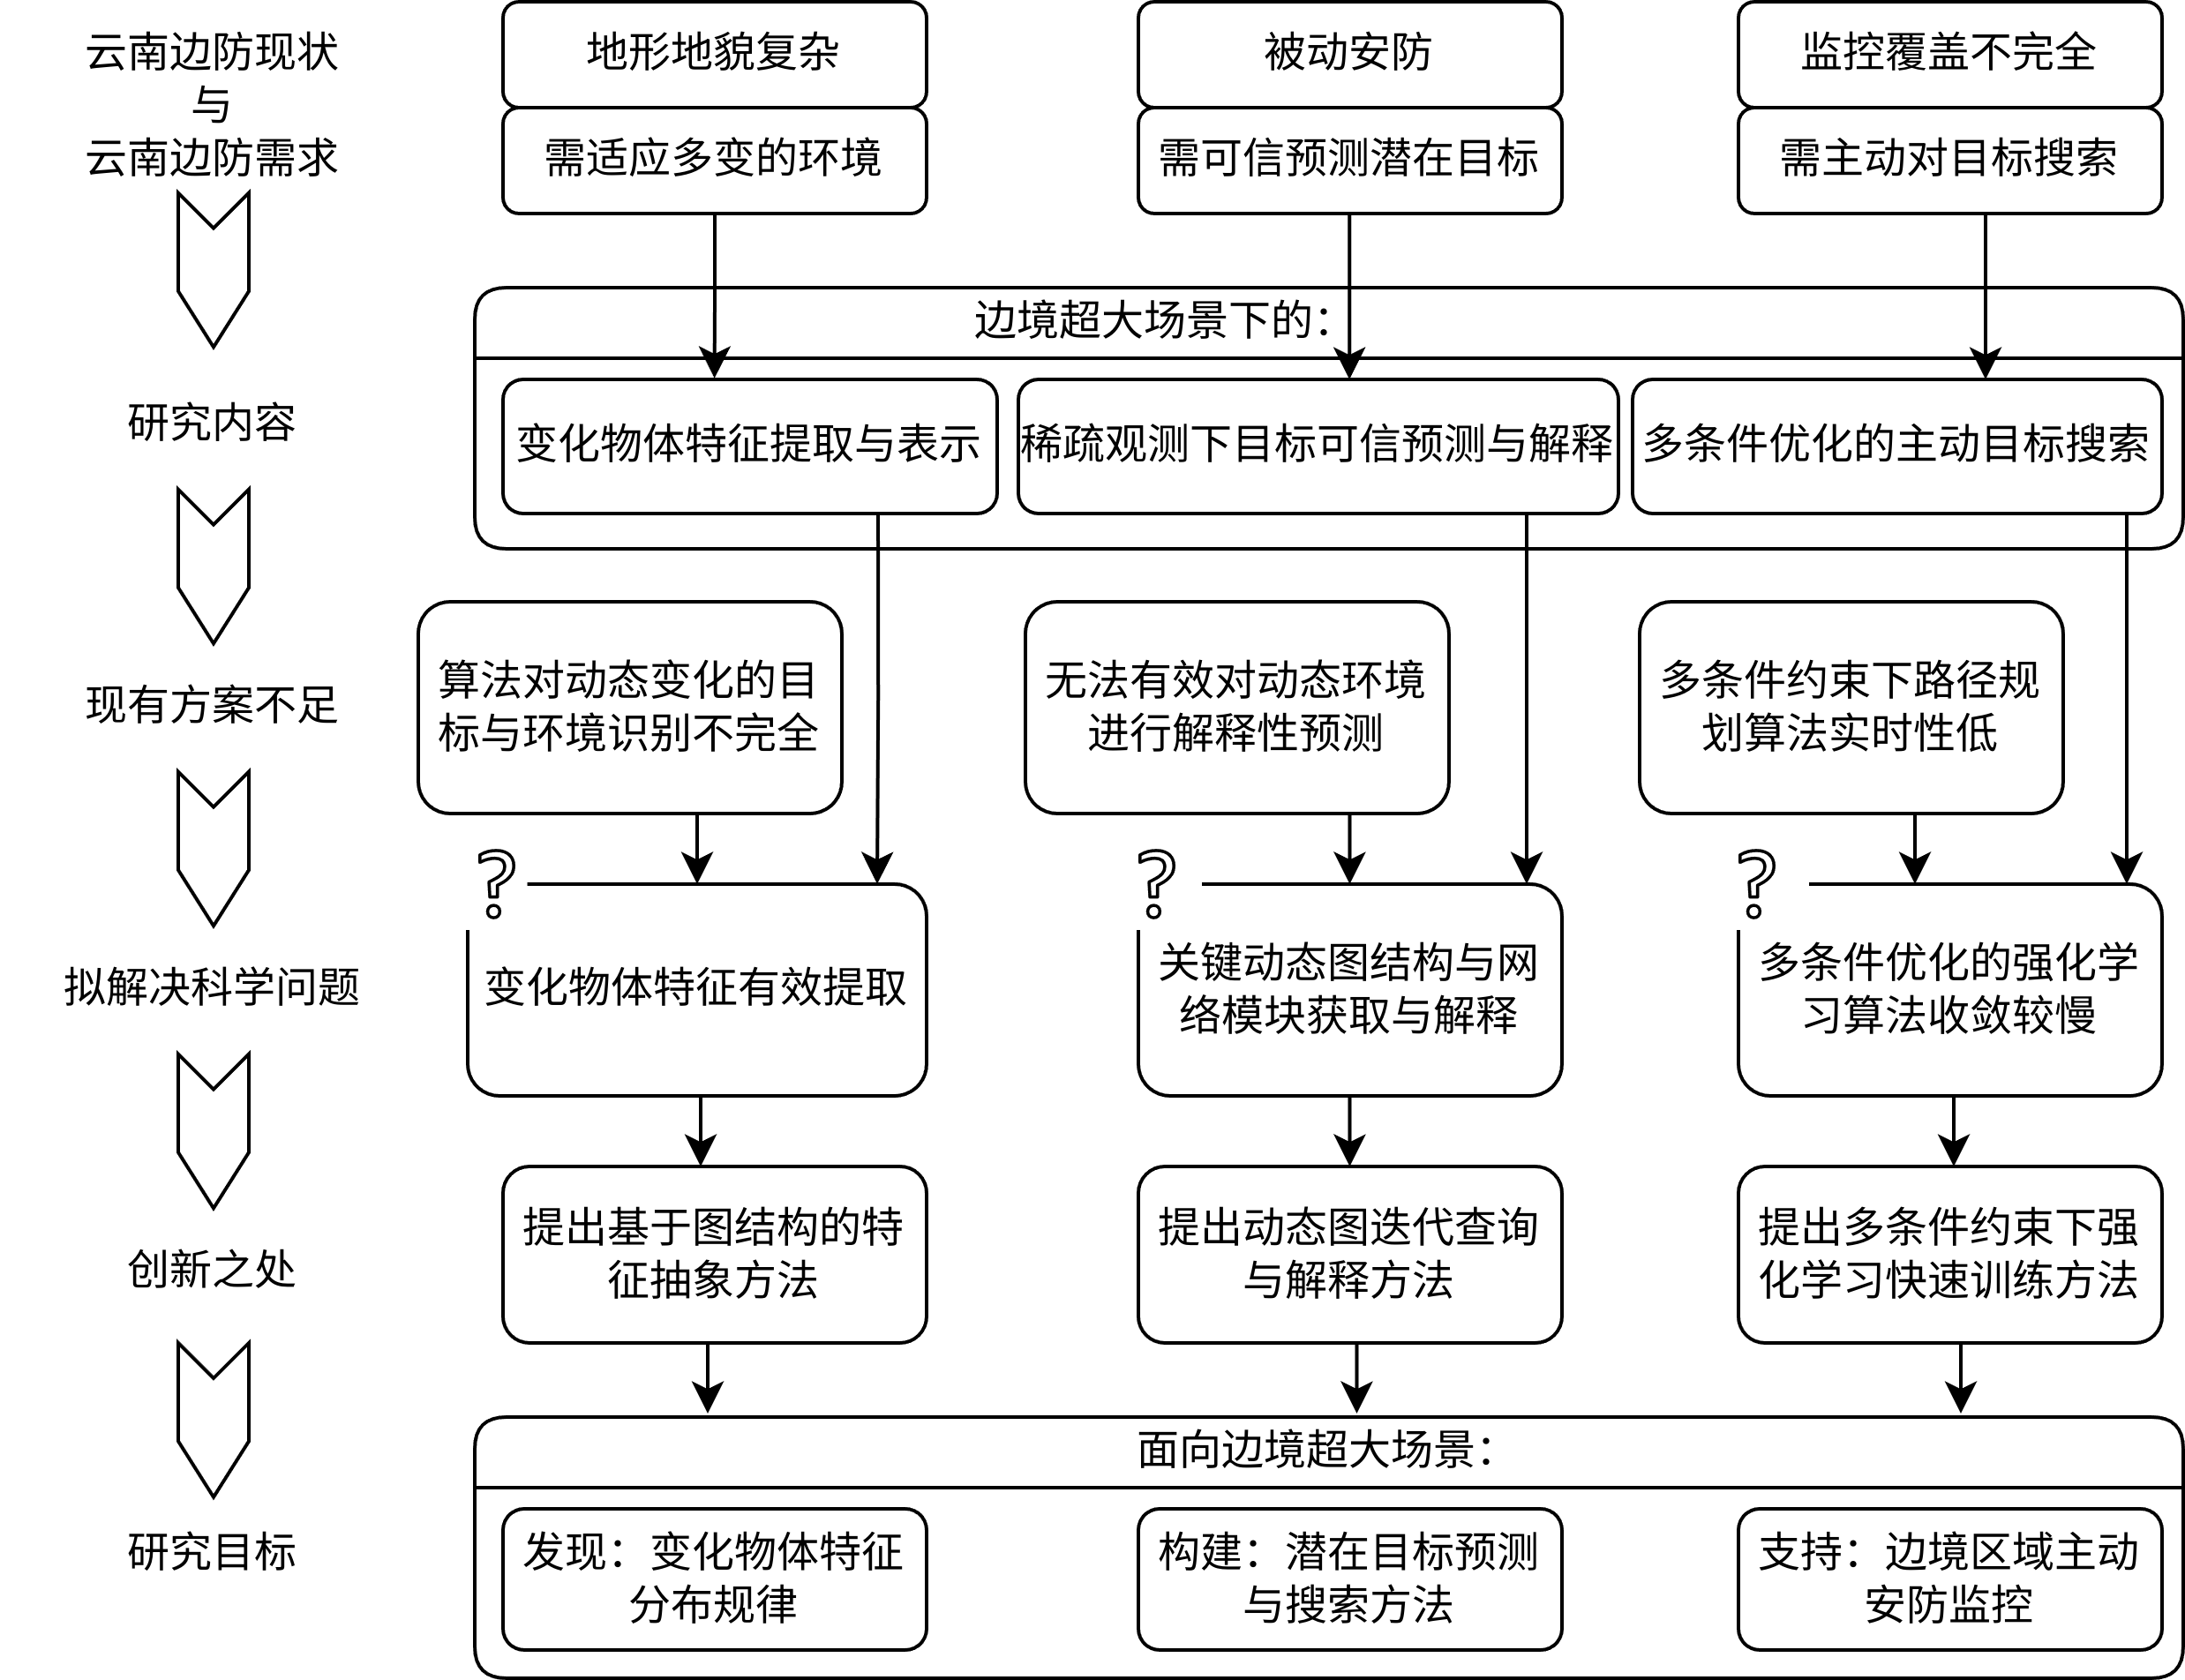
\includegraphics[width=1\textwidth]{2-1}
\captionsetup{justification=centering}
\caption{组织结构}
\label{fig:organization}
\end{figure}

\subsection{研究内容}



\subsubsection*{\bfseries (1)超大场景下变化物体特征提取与表示方法研究}
物体特征的有效提取与表示是后续目标预测与主动搜索的前提,其目的是为后续过程提供不受环境因素和场景变化影响的物体特征表示。在超大场景下,同一物体的特征往往那个会受到光照,天气,周围物体遮挡或物体本身的形态变化而产生较大变化,使得该物体不能有效被视觉模型识别和理解。
因此,\textbf{研究物体特征抽象与分离方法,使复杂变化对物体特征的影响最小化。一方面,将物体内在的固有特征和物体受到外界因素变化显现的外在特征相分离,另一方面,使用对比学习等手段进一步同化相同物体的表示,异化不同物体的表示,以实现对变化物体的成功识别和理解}。
由此解决现有方法对超大场景下变化物体特征提取的困难,为后续目标的预测和主动搜索提供稳定可到的物体表示。


\subsubsection*{\bfseries (2)超大场景稀疏观测下的目标位置可信预测与解释方法研究}
目标位置可信预测根据当前摄像设备的局部观测信息推断目标物体在超大场景内位置的概率分布。
摄像设备的局部观测往往具有稀疏性,因为单一监控设备往往不能全面清晰的获取超大场景任意时刻的全景,仅能够观测并获取其中的一个子区域的信息。
目标可信预测的目的是为后续目标主动搜索提供必要依据,否则搜索过程将冗余和低效,降低目标发现的可能性。
预测的目标位置依赖于当前观测的信息,但由于数据噪声和环境物体的不确定性,需要必要的可解释机制描述目标潜在位置的可信度。
因此,\textbf{研究观测与物体潜在位置之间的条件依赖关系,针对超大场景下的观测的稀疏性问题,重点研究当前观测物体对潜在目标之间的条件分布变化规律,探索并发现依赖关系背后的可解释性原理,为全数据流程各个各个环节的构建提供依据}。


\subsubsection*{\bfseries (3)超大场景下多条件约束的主动目标搜索方法研究}

主动目标搜索的目的有两个方面。首先,利用自动智能算法代替现有被动人工介入的监控模式,实现全天候监控覆盖;其次,利用单一超大场景主动搜索机制代替同能监控能力下大量被动监控设施。从而双管齐下的节约成本并提升监控能力。现有主动搜索方法主要采用区域覆盖的方式排查目标,对于超大场景下的动态目标搜索能力有限。
因此,\textbf{研究超大场景下动态目标的主动搜索,针对监控设备在调整转动角,俯仰角及变焦时的物理噪声和精度问题,重点研究自适应的控制方法,依据潜在目标的位置,通过序列化决策主动搜索并发现目标},解决现有方法存在的困难。


\subsection{研究目标}

本课题拟通过构建\textcircled{1}超大场景下变化物体特征提取与表示方法;
\textcircled{2}超大场景下基于稀疏观测的目标位置预测与可解释方法;\textcircled{3}超大场景下主动目标搜索方法方法,拟达到以下目标:
(1)发现变化物体特征之中的通用特征,进而深度模型对动态超大场景内物体的范化能力和稳定性;(2)提出观测条件受限情况下的特定目标在超大场景中的潜在位置可信预测与主动搜索方法,将当下边境安防监控的被动监视状态转变为主动监控状态,提前对潜在目标进行响应;(3)搭建实验平台、构建公开数据集、开发原型系统以提升研究深度广度、促进学术交流与技术应用落地。

\subsection{拟解决的关键科学问题}

上述研究内容在解决现有方法面对的困难和挑战时,主要需解决如下关键科学问题。


\subsubsection*{\bfseries (1)超大场景下变化物体图像特征提取有效性受环境变化显著下降的问题}
在图像特征提取过程中,现有基于CNN的方法通过多层卷积操作提取物体特征,每一层卷积核能够捕捉图像中的局部特征(如边缘、纹理等),并通过堆叠多层网络逐步提取更高层次的语义信息(如形状、结构等)。
然而在不断变化的超大场景下,物体的轮廓,边缘等关键信息往往会发生显著变或表现为较强的环境噪声。
CNN对噪声敏感,原因在于其卷积操作本质上是对局部像素的加权求和,噪声会直接干扰局部像素值,导致特征提取的偏差。同时,噪声可能在高层次特征中被放大,进一步影响模型的分类或检测性能。因此,噪声的存在会降低CNN特征提取的鲁棒性和准确性。
基于Transformer的视觉模型虽然考虑到了细微像素点特征长距离依赖关系,但仍然无法有效处理较大的物体变化,对环境噪声依然较为敏感,原因与CNN模型类似。
因此,为了避免单一局部特征受到噪声影响导致的模型误判,\textbf{本项目拟对物体特征进行抽象,提取和利用不用变化下统一物体固有的不变特征,由此便能够准确识别物体。同时,辅以物体随环境变化的特征,便能够在正确识别物体的前提下,充分考虑原始局部特征},为后续预测提供更加全面细致的特征。
% 本研究充分考虑到细微特征随环境显著变化的特点,发现需要从宏观特征出发,对观测的信息进行抽象,将其分为全局结构特征和局部细节特征,利用现有视觉分割方法在低精度条件下提取宏观结构,借助关系模型学习宏观结构内的全局特征;接着再利用局部特征对全局特征进行补充,从而避免了仅利用单一局部特征造成的模型误判


\subsubsection*{\bfseries (2)超大场景下动态特征学习过程中关键图结构与模型网络模块的获取与解释问题}
超大场景通常具有数据规模庞大、环境复杂多变、目标动态性强等特点,这对特征学习的实时性、鲁棒性和可解释性提出了极高的要求。首先,超大场景中的数据流通常具有高维度和高复杂性的特点,传统特征学习方法难以有效捕捉数据中的动态变化。例如,在边境安防过程中,植物、动物、道路状况等目标的动态变化需要实时捕捉和分析,这对特征学习的实时性和鲁棒性提出了更高要求。其次,动态特征学习的可解释性问题尚未得到充分解决。深度学习“黑箱”特性使得特征提取过程缺乏透明性,难以解释模型决策的依据,这在边境安防监控等安全敏感领域中尤为关键。
\textbf{本项目拟提出一种基于动态图神经网络(Dynamic GNN)和可解释性人工智能(XAI)技术的动态特征学习方法。}首先,利用动态图神经网络对超大场景中的数据流进行建模,通过图结构的动态更新捕捉目标之间的时空关系,提升特征学习的鲁棒性和适应性。其次,结合可解释性人工智能技术,对特征提取过程进行可视化分析,揭示模型决策的关键因素,增强模型的可解释性和可信度。此外,通过设计轻量化的特征学习框架,降低计算复杂度,满足超大场景下的实时性需求。最后,通过实验验证该方法在复杂场景下的性能,并与现有方法进行对比,展示其在特征学习精度和可解释性上的优势。

\subsubsection*{\bfseries (3)超大场景与多条件约束下的强化学习算法收敛性问题}

超大场景下多条件约束的主动搜索问题是智能监控等领域的核心挑战之一,其目标是在复杂环境中高效搜索和发现目标。传统搜索方法在超大场景下面临搜索空间大、目标分布稀疏以及多条件约束的挑战,导致效率低下。大空间搜索往往需要遍历的区域广阔,计算复杂度高;目标分布稀疏则增加了定位目标的难度,容易产生大量无效搜索。此外,多条件约束(如时间、资源限制和环境动态变化)进一步限制了搜索的灵活性和适应性,使得传统方法难以在复杂场景中高效完成任务。
因此,\textbf{本项目拟使用基于强化学习的主动搜索方法,通过智能体间的信息共享与协作,动态调整搜索策略以应对多条件约束。} 针对训练过程,需要设计合理的训练方法帮助模型在有限的资源下收敛。为了更好的适应物理监控设备的操控特性,研究将进一步优化多条件约束下的搜索策略,推动该技术在边境安防监控领域的应用。